\begin{frame}{Evaluation und Metriken}
\small
\begin{columns}[T,onlytextwidth]
\begin{column}{0.46\textwidth}
\begin{tabular}{lrr}
\toprule
Einstellung & Red20 & Red6/10 \\
\midrule
Validierungsbilder & 300 & 500 \\
GT-Faces & 3.443 & 5.015 \\
IoU-Schwelle & 0,4 & 0,4 \\
Confidence & 0,25 & 0,25 \\
\bottomrule
\end{tabular}
\end{column}
\begin{column}{0.5\textwidth}
\begin{itemize}
    \item Recall macht Datenschutzrisiko messbar.
    \item Treffer zeigen die absolute Groessenordnung.
    \item Precision und F1 helfen bei der Threshold-Wahl.
    \item ms/Bild entscheidet ueber Videotauglichkeit.
\end{itemize}
\end{column}
\end{columns}
\vspace{0.5em}
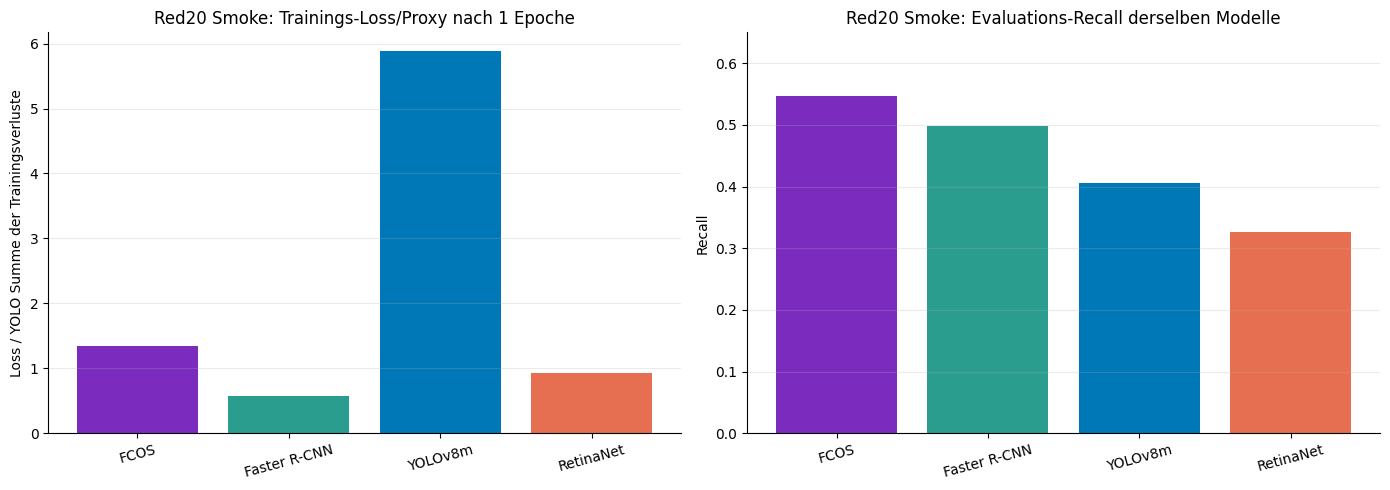
\includegraphics[width=\textwidth,height=0.34\textheight,keepaspectratio]{imglib/face_model_lab/red20_training_vs_eval.png}
\end{frame}
